% Template for ICASSP-2020 paper; to be used with:
%          spconf.sty  - ICASSP/ICIP LaTeX style file, and
%          IEEEbib.bst - IEEE bibliography style file.
% --------------------------------------------------------------------------
\documentclass{article}
\usepackage{spconf,amsmath,graphicx, hyperref} %

% Example definitions.
% --------------------
\def\x{{\mathbf x}}
\def\L{{\cal L}}

% Title.
% ------
\title{Using 1D convolutional neural network (CNN) to classify audio frequencies}
%
% Single address.
% ---------------
\name{Chad Kakau \thanks{AIML425}}
\address{Victoria University, Wellington}
%
%
\begin{document}
%\ninept
%
\maketitle
%
\begin{abstract}
This paper develops a simple 1D convolutional neural network to learn and classify audio signals.  The paper briefly summarises the 1D convolutional neural network, in particular the effects of pool sizes, and stride length on CNN performance.  Implementing a simple 1D CNN results in better validation and test results for smaller pool sizes and shorter stride lengths.  Implementation also includes reviewing a mixture of frequencies (summation of two fundamental frequencies), that results in comparable performance to the single frequency models at highest stride length and pool sizes.  The paper concludes by acknowledging the relative simplicity (i.e. repepetitive and constant wave form) of the reference frequencies leads to good performance of the CNN, before considering testing the model on more complex signals in the future.
\end{abstract}
%
\begin{keywords}
1D Convolutional neural network, 1D CNN
\end{keywords}
%
\section{Introduction}
\label{sec:intro}
%
Neural networks continue to provide state of the art results for image and audio recognition applications \cite{brownlee_1d_2018} including classification.  1D CNN uses input data that can be traversed in a single direction, so audio files make excellent candidates for machine learning models \cite{noauthor_convolutional_nodate}.  By combining with a range of other neural network methods, we can implement quite complex models for any range of tasks, in this case for classification of noisy audio signals into one of five frequencies.  This implementation will generate five reference signals as 2 second tonal frequencies, then add noise to the data before applying a 1D CNN, a pooling layer, flattening the data and then creating two dense layers, the first with 64 nodes, the second and final layer, with five nodes, each representing one of the five reference frequencies.

\section{Audio signals and 1D CNNs}
\label{sec:format}

For this implementation we begin by generating reference frequencies for use as the class or label items. Then we will put those frequencies through a 1D CNN, adjusting stride length and pool size to tune the model's performance.

\subsection{Audio and Hamming window}
\label{ssec:audio}
At its most basic, an audio signal can be represented as an array of numeric values, each indicating a quantity of energy received (or sent) at a specific time \cite{noauthor_audio_nodate}.  Humans can perceive audio frequencies between $15 - 20000$Hz \cite{Kulkarni_human}, with that perception deteriorating with age, especially for higher frequencies.  

Because we will feed the audio signals into a neural network, we need to ensure that each signal has the same shape (i.e. number of time-steps or sample points, and the same number of channels) \cite{noauthor_audio_nodate}.  We can achieve this using a window function, in this case we will use a Hamming window, which is represented as a known length (of time-steps), tapering cosine curve with tails $>1$ \cite{noauthor_use_nodate} \cite{harris_multirate_1987}.  By combining a Hamming window with a frequency we can generate an output array of a known length, that can be converted to a soundfile  \cite{noauthor_05-frequency-analysis_nodate}.  To generate the output frequency we multiply our Hamming wndow by $\sin ( \omega t)$, where $ \omega = 2 \pi f $, where $ f $ is the input frequency.  $ \omega$ is also known as the "angular frequency".  

We take the following frequencies:

$f \in {317Hz, 780, 1234Hz, 2017Hz, 3106Hz}$  

\subsection{Stride length and pooling}
\label{ssec:stride}

In this 1D CNN we will tune to key parameters:  stride length and pool size.  The 1D CNN passes a filter across the input array, the filter performs some function against each element in its area and outputs the result of that function to the next layer \cite{noauthor_convolutional_nodate}.  The filter may pass one element at a time (so a 3-bit filter will cover each element three times), giving a stride length of 1, or it may pass across the element faster by taking longer strides.  This increases the speed at which the filter processes the array but also reduces the amount of information available to the next and subsequent layers in the model.  

Pooling is a technique where a group of elements are represented by some feature of that group, usually the max value or the average.  Max pooling allows for the detection of a feature, but may not provide detail as to the location of that filter within the pool.  Again, pooling reduces the amount of information available to subsequent layers, but brings an increase in speed.  We should expect performance to degrade as the stride length and pool size increases \cite{noauthor_convolutional_nodate}.

For the purpose of comparison, we present these five frequencies in two ways: the upper plots show amplitude (y axis) over time (x axis) and the plots all have the same time scale.  The lower plots show the fast fourier transformation of each frequency, this time with frequency along the x axis, showing a clear spike at the relevant frequency.  Using fast fourier transformation allows us to decompose a complex signal into its component parts and can be useful for identifying the contributing frequencies in order to isolate and amplify or filter that frequency \cite{noauthor_05-frequency-analysis_nodate}.

\begin{figure}[htb]
\begin{minipage}[b]{1\linewidth}
  \centering
  \centerline{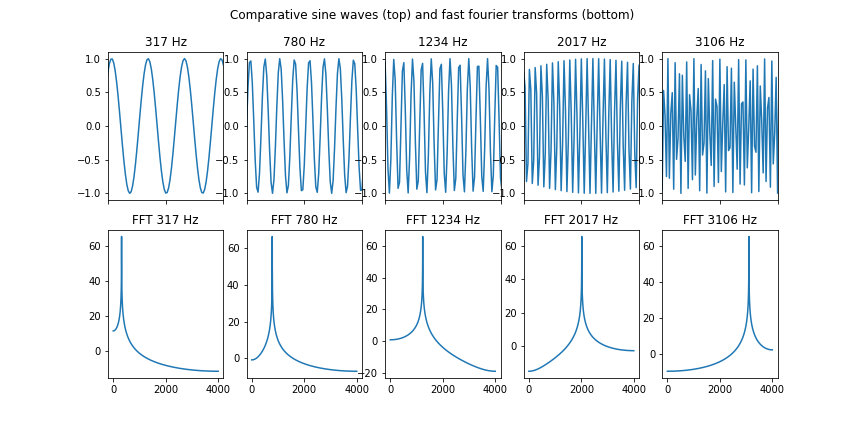
\includegraphics[width=8.5cm]{sine_fft_main}}
%  \vspace{2.0cm}
\caption{"Initial frequencies and fast fourier transforms"}
\label{fig:sin_fft}
\end{minipage}
\end{figure}
%

(Fig \ref{fig:sin_fft}) shows the first five frequencies and should be compared against the later plot showing mixed frequencies (Fig \ref{fig:mixed})
:

\begin{figure}[htb]
\begin{minipage}[b]{1\linewidth}
  \centering
  \centerline{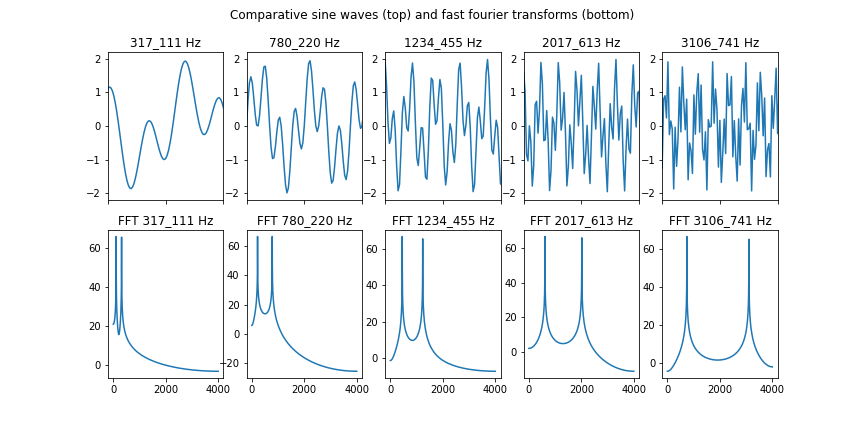
\includegraphics[width=8.5cm]{sine_fft_mixed}}
%  \vspace{2.0cm}
\caption{"Mixed frequencies and fast fourier transforms"}
\label{fig:mixed}
\end{minipage}
\end{figure}

\section{RESULTS}
\label{sec:results}
%
The results show that the 1D CNN can learn to classify audio signals with very high accuracy, including when using quite high stride length and pool size.  

%  \vspace{2.0cm}
\begin{figure}[htb]
\begin{minipage}[b]{.48\linewidth}
  \centering
  \centerline{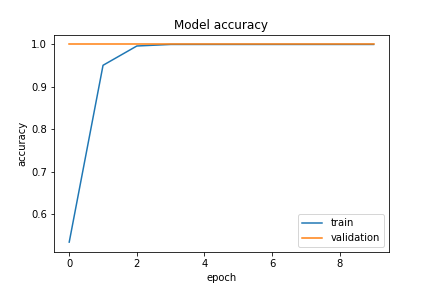
\includegraphics[width=4cm]{pool2}}
  \centerline{(a) Pool = 2, stride = 100}
\end{minipage}
\begin{minipage}[b]{.48\linewidth}
  \centering
  \centerline{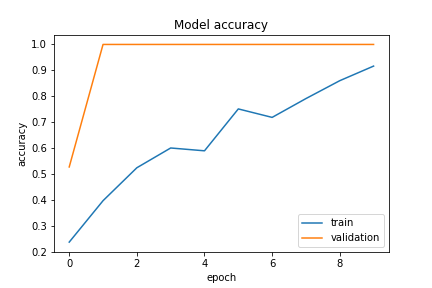
\includegraphics[width=4cm]{pool8}}
  \centerline{(b) Pool = 8, stride = 100}
%  \vspace{2.0cm}
\end{minipage}
%
\caption{Performance of 1D CNN with different pool size}
\label{fig:res1_2}
%
\end{figure}

We compare performance of 1D CNNs, with strides of the same length (8) and pool = 2, then pool 8 (Fig \ref{fig:res1_2}).  We can see that performance with a smaller pool size (i.e. pooling fewer elements) is better than with a larger pool.  The training accuracy improves at a slower rate for pool = 8 and never reaches the full accuracy in the model.  Validation and test results for both models reach 100\% early.  

\begin{figure}[htb]
\begin{minipage}[b]{0.48\linewidth}
  \centering
  \centerline{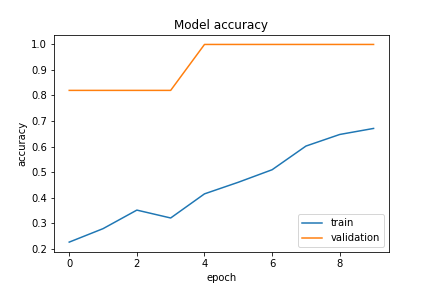
\includegraphics[width=4cm]{strides180_pool8}}
  \centerline{(c) Pool = 8, stride = 180}
%  \vspace{1.5cm}
\end{minipage}
%
\begin{minipage}[b]{0.48\linewidth}
  \centering
  \centerline{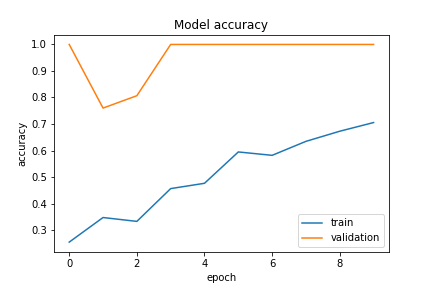
\includegraphics[width=4cm]{mixed}}
  \centerline{(d) Pool = 8, stride = 180}
%  \vspace{1.5cm}
\end{minipage}
%
\caption{Performance with strides of 180 and mixed frequencies}
\label{fig:res3_4}
%
\end{figure}

We can also compare the results of models with pool = 8, stride = 180 but using the baseline frequencies versus mixed frequencies. (Fig \ref{fig:res3_4}) shows very similar performance for both models, both reaching maximum training accuracy of around 60\% after 10 epochs of training, but with validation accuracy at 100\% by the fourth epoch and test accuracy of 100\%.

\hfill

\section{CONCLUSION}
\label{sec:CONC}

1D CNN performance on predicting 1-channel audio tones appears to be dependent on stride length and pool size, and performs comparably when comparing either a single sinusoidal tone or a complex combination of two sinusoid waves.  The effect of stride length seems fairly intuitive, since the length of each stride determines either how many times an element is sampled by each filter on each pass (i.e. low stride length) or how many individual elements may be missed altogether (i.e. high stride length) by each filter on each pass.  For an array of the nature and size in this implementation, the stride length can become quite large before training accuracy is noticably degraded.  

The effect of increased pool size is more readibly noticed when downstream from increased stride length because as information is lost (i.e. the filter strides past elements) there are fewer elements to pool and key feature elements (e.g. peaks and troughs) of the underlying array may be lost or missed, making learning more challenging.  The trade-off for loss of information is reduced computation (due to fewer elements), resulting in faster models.  

It would be interesting to test a model against more complex or erratic audio signals (e.g. ambient noise on the street to detect vehicle types, or birdsong to classify birds in a neighbourhood etc.), similar to the models generated at \cite{brownlee_1d_2018} and \cite{noauthor_simple_nodate}.  A 1D CNN in these situations should provide very useful results, although tuning would likely result in degraded performance at lower stride and pool values, which should in turn bring longer processing times.  

Link to colab site for code: 

\url{https://colab.research.google.com/drive/13lFG3ZxG-QAvMwT4B3hzLTMdNQNgMAkG?usp=sharing}

\bibliographystyle{IEEEbib}
\bibliography{references}

\end{document}
